% Name: Waffle chart
% Description: A grid of 100 squares, one for each percent of survey answers, colored 58 yes, 27 no, and 15 unsure.
% Tags: waffle chart, percentages, survey, proportions

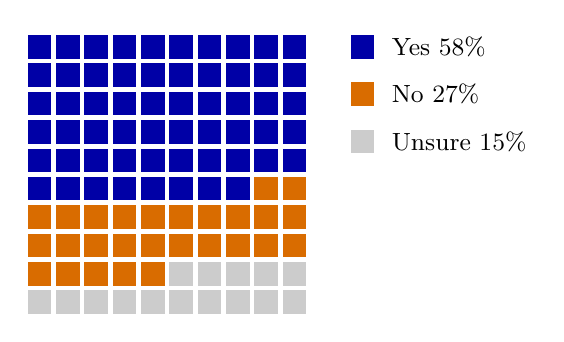
\begin{tikzpicture}[font=\small]
  % Squares are counted row by row from the top left: 0 to 57 yes, 58 to 84 no, and 85 to 99 unsure.
  \foreach \i in {0,...,99} {
    \pgfmathtruncatemacro\col{mod(\i,10)}
    \pgfmathtruncatemacro\row{\i/10}
    \ifnum\i<58 \def\c{blue!65!black}\else\ifnum\i<85 \def\c{orange!85!black}\else \def\c{gray!40}\fi\fi
    \fill[\c] (0.36*\col, -0.36*\row) rectangle ++(0.3,0.3);
  }
  \foreach \name/\c [count=\i from 0] in {Yes 58\%/blue!65!black, No 27\%/orange!85!black, Unsure 15\%/gray!40} {
    \fill[\c] (4.1,-0.6*\i) rectangle ++(0.3,0.3);
    \node[anchor=west] at (4.5,-0.6*\i+0.15) {\name};
  }
\end{tikzpicture}
